\chapter{Práticas corporais: dos jogos eletrônicos aos esportes radicais}
\markboth{Módulo 1}{}

%Felipe: quando havia problemas gramaticais nos textos utilizados (o que não foi incomum), fiz a correção e coloquei a expressão ``com alterações'' depois da citação. Em um dos textos, o autor suprimiu uma alusão a Dilma Roussef, mas essa supressão comprometia a compreensão do texto. Mantive a supressão, mas fiz pequena adaptação.    

\section{Habilidades do SAEB}

\begin{itemize}
\item
  Identificar as diferentes valências físicas necessárias
  à realização de práticas corporais (jogos eletrônicos, lutas, práticas
  corporais de aventura, ginásticas, esportes e dança).
\item
  Identificar o valor do patrimônio urbano e natural nas vivências das
  práticas corporais de aventura urbana e na natureza.
\item
  Identificar as características (códigos, rituais, elementos
  técnico-táticos, indumentária, materiais, instalações, instituições)
  das lutas.
\item
  Analisar as práticas corporais frente à disponibilidade de locais para
  sua vivência.
\item
  Analisar as transformações históricas, o processo de esportivização e
  a midiatização das práticas corporais, com ênfase nas lutas.
\end{itemize}

\section{Habilidades da BNCC}

\begin{itemize}
  \item
EF67EF01, EF67EF06, EF89EF03, EF89EF15, EF89EF18
\end{itemize}

%\reversemarginpar\marginnote{O objetivo deste módulo é habilitar o estudante a entender o processo de esportivização e identificar as práticas corporais presentes na sociedade, reconhecendo suas principais características, e as valências físicas presentes nas modalidades esportivas.\\}

\conteudo{As práticas corporais (jogos eletrônicos, ginásticas esportes, lutas,
danças etc.) são manifestações corporais presentes na sociedade. Em cada uma dessas atividades são trabalhadas as \textbf{valências físicas}, que são: \textbf{força} (vencer uma
carga externa), \textbf{velocidade} (realizar um movimento no menor
tempo possível), \textbf{resistência} (realizar o mesmo movimento por
vários segundos) e \textbf{flexibilidade} (capacidade de esticar uma
musculatura ao máximo).

Além disso, muitas práticas passam por um processo de \textbf{esportivização}, ou
seja, deixam de ser uma atividade voltada para o lazer e passam a ser um
esporte oficial. Suas características são:

\begin{itemize}
\item
  Presença de regras oficiais padronizadas;
\item
  Criação de órgãos oficiais para fiscalizar o esporte (federação e
  confederação);
\item
  Competições oficiais e treinamentos específicos.
\end{itemize}
}

\section{Atividades}

\num{1} Escreva as capacidades físicas mais utilizadas em cada prática corporal:

\begin{escolha}
\item
  Corrida dos 100 metros: \reduline{velocidade.\hfill}
\item
  Maratona: \reduline{resistência.\hfill}
\item
  Ginástica artística: \reduline{flexibilidade.\hfill}
\item
  Levantamento olímpico: \reduline{força.\hfill}
\end{escolha}

%\coment{Por meio desta atividade, o estudante vai poder relacionar e identificar as capacidades físicas utilizadas em algumas práticas corporais.}

\num{2} Relacione o tipo de práticas corporais de aventura (urbana ou
  natureza) com as modalidades apresentadas a seguir.

\begin{enumerate}
\item Prática de aventura urbana

\item Prática de aventura na natureza
\end{enumerate}

\begin{boxlist}

\boxitem{1} Slackline

\boxitem{2} Moutain bike

\boxitem{2} Corrida de orientação

\boxitem{1} Skate
\end{boxlist}

%\coment{O objetivo desta atividade é habilitar o estudante a distinguir as práticas corporais realizadas nos ambientes urbanos das que ocorrem na natureza, valorizando os espaços para essas modalidades.}

\num{3} Observe a imagem a seguir:

\begin{figure}[htpb!]
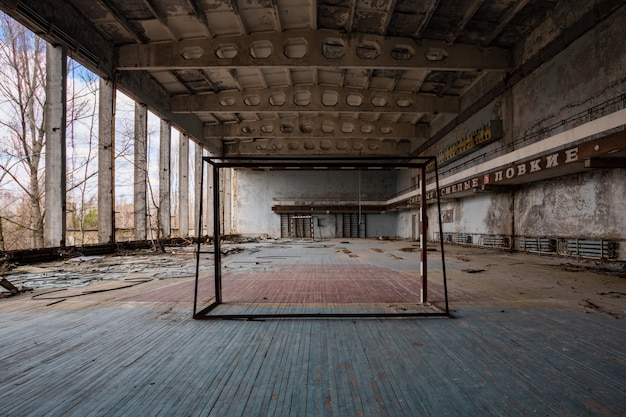
\includegraphics[width=2.99444in,height=1.99477in]{./imgs/img1.jpg}
%\caption{Fonte: https://br.freepik.com/fotos-gratis/ginasio-abandonado-em-pripyat\_13499703.htm\#query=parque\%20abandonado\&position=6\&from\_view=search\&track=ais}
\end{figure}

Observando a imagem, é possível realizar alguma prática corporal? Qual é
o nosso dever em relação a esses espaços.

\reduline{Na imagem, observa-se um ginásio esportivo abandonado, de
infraestrutura comprometida, cujo abandono, além de oferecer riscos
à saúde dos esportistas, inviabiliza o uso pela comunidade. O papel
das pessoas é preservar espaços públicos como esse, que podem ser 
extremamente benéficos quando adequadamente utilizados.
O propósito desta atividade é estimular o espírito crítico 
dos estudantes no que concerne aos espaços públicos disponíveis
na cidade.\hfill}

\num{4} No passado, o judô era uma luta voltada para a defesa pessoal.
  Atualmente é uma modalidade olímpica dividida em categorias, com 
  distinção de golpes proibidos e legítimos. É possível afirmar que essa
  luta passou por um processo de esportivização? Justifique sua
  resposta.

  %É adequado chamar o judô de "luta"? Minha experiência em escolas me ensinou que a expressão "arte marcial" é mais adequada (mas pode ser ignorância minha). (Rogério, 6/4/23, 13h08)

\reduline{É correto afirmar que o judô passou pelo processo de
esportivização, pois, embora tenha sido um luta voltada para a autodefesa,
hoje em dia é um esporte com categorias, regras e golpes padronizados,
que são realizados em competições oficiais, como as Olimpíadas.
O objetivo dessa atividade é que o estudante
compreenda o processo por meio do qual uma prática corporal se torna 
um esporte oficial.\hfill}

\section{Treino}

\num{1} Observe a imagem a seguir:

\begin{figure}[htpb!]
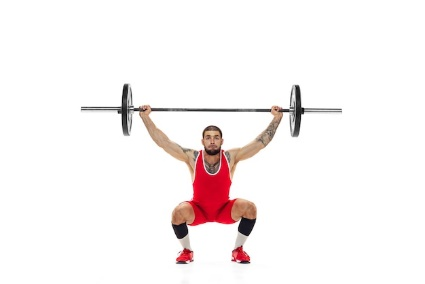
\includegraphics[width=1.92222in,height=1.28367in]{./imgs/img2.jpg}
%\caption{Disponível em: https://br.freepik.com/fotos-gratis/jovem-esportivo-treinando-com-barra-de-peso-isolada-sobre-fundo-de-estudio-branco-situps\_24908397.htm\#query=levantamento\%20de\%20peso\&position=41\&from\_view=search\&track=ais}
\end{figure}

Com base na imagem, o atleta está praticando uma modalidade que trabalha
a valência física de

\begin{escolha}
\item força, pois está vencendo uma carga externa que são as anilhas.

\item resistência, pois ficar agachado exige contração muscular das pernas.

\item velocidade, pois deve-se pegar a barra no chão e levantá-la para
cima.

\item flexibilidade, pois os músculos dos braços estão esticados.
\end{escolha}

\num{2} Leia o texto a seguir:

\begin{quote}
O município de Salvaterra, no arquipélago paraense do Marajó, será palco
da estreia da luta marajoara nos Jogos Estudantis Paraenses (Jeps).

{[}...{]}

A típica luta marajoara é um combate corpo a corpo, que tem o objetivo
de projetar o oponente de costas ao chão e dominá-lo, esporte semelhante
ao Wrestling, praticado no norte do Brasil. Esta é a primeira vez que a
modalidade é incluída no torneiro, que está na sua 62ª edição.

\fonte{GE Pará. Salvaterra recebe os primeiros combates da luta marajoara
como modalidade do Jeps. Disponível em:
https://ge.globo.com/pa/noticia/salvaterra-recebe-os-primeiros-combates-da-luta-marajoara-como-modalidade-do-jeps.ghtml
. Acesso em: 6 abr. 2023.}
\end{quote}

Com base no texto, pode-se afirmar que a luta marajoara passou
por um processo de esportivização porque

\begin{escolha}
\item foram criados órgão oficiais relacionados a essa prática.

\item a prática está presente em um evento oficial.

\item o objetivo da prática foi alterado para a competição.

\item essa prática se assemelha à de um outro esporte.
\end{escolha}

\num{3} Leia o texto a seguir:

\begin{quote}
Skatistas de Curitiba terão, em breve, um novo espaço para praticar o
esporte. A Prefeitura de Curitiba começará a construir nos próximos 15
dias a maior pista pública de skate da cidade 

A pista, de 450 metros quadrados, será a primeira da região e é uma antiga 
reivindicação da população. O projeto feito pela Secretaria Municipal do 
Meio Ambiente teve a participação de skatistas. "Tomamos os cuidado de 
ouvir os praticantes do esporte e deixar o projeto o mais próximo possível 
da necessidade dos usuários", conta o superintende de obras e serviços da 
secretaria, Paulo Dalmaz.

%Felipe: consultei o original e alterei o trecho do texto escolhido. Na questão originla, a alternativa correta estava baseada em uma inferência duvidosa; entendo que, agora, a questão ficou mais consistente, além de enfatizar a demanda da população pelo esporte. (Rogério, 6/4/23, 13h45)

\fonte{Prefeitura Municipal de Curitiba. Nova pista pública de skate
será a maior da cidade. Disponível em:
https://www.curitiba.pr.gov.br/noticias/nova-pista-publica-de-skate-sera-a-maior-da-cidade/7410. Acesso em: 6 abr. 2023.}
\end{quote}

Após a leitura do texto, pode-se afirmar que o objetivo da construção da 
pista pública de skate é

\begin{escolha}
\item formar novos atletas para competições oficiais.

\item incentivar o uso de um novo meio de transporte.

\item atender à demanda da população pela prática do skate.

\item criar novos investimentos financeiros para a prefeitura.
\end{escolha}

\chapter{Esporte e dança}
\markboth{Módulo 2}{}

%\coment{O objetivo deste módulo é que o aluno compreenda as definições dos esportes e entenda as características das danças, especificamente das danças urbanas.\\

\section{Habilidades do SAEB}

\begin{itemize}
\item
  Diferenciar os esportes com base nos critérios de sua lógica interna.
\item
  Diferenciar as danças urbanas, seus elementos constitutivos e seu
  valor cultural nas demais manifestações da dança.
\end{itemize}

\section{Habilidades da BNCC}

\begin{itemize}
\item EF67EF12, EF67EF13.
\end{itemize}

\conteudo{As \textbf{danças urbanas} desenvolveram-se em centros
urbanos ou periferias como forma de expressão e crítica social, por meio
do uso do corpo. É o caso da cultura do hip hop, que abarca traços
de diversas culturas e traz muitos benefícios para o praticante.

Além disso, muitas dessas danças, como o \textbf{breaking}, estão passando
pelo processo de esportivização e vão fazer parte de eventos oficiais,
como as Olimpíadas.}

\section{Atividades}

\num{1} Observe os elementos do hip hop numerados de 1 a 4 e preencha os quadrados com suas respectivas características.

\begin{enumerate}
\item Rap

\item Breaking

\item Grafite

\item DJ
\end{enumerate}

\begin{boxlist}
\boxitem{2} Dança do hip hop em que o dançarino pode improvisar os movimentos.

\boxitem{3} Desenhos artísticos feitos em muros ou em paredes com spray.

\boxitem{1} Canção do hip hop que tem improvisações e rimas.

\boxitem{4} Pessoa responsável pela mixagem do som.
\end{boxlist}

%\coment{ O objetivo dessa atividade é que o aluno identifique os elementos da cultura do hip hop.}

\num{2} Observe a imagem a seguir:

\begin{figure}[htpb!]
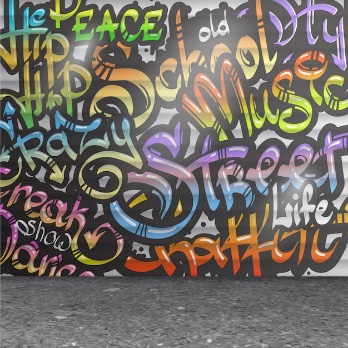
\includegraphics[width=1.57407in,height=1.57407in]{./imgs/img3.jpg}
\caption{Fonte: https://br.freepik.com/vetores-gratis/fundo-da-parede-de-graffiti\_4631697.htm\#page=2\&query=hip-hop\&position=47\&from\_view=search\&track=sph}
\end{figure}

Podemos dizer que a imagem mostra uma pichação? Justifique sua resposta.


\reduline{Na imagem, observa-se não uma pichação, mas um grafite. 
O grafite é uma forma de arte visual cujos desenhos são feitos com spray,
normalmente realizados com autorização de prefeituras ou donos de
estabelecimentos. As pichações, por sua vez, são formas de vandalismo.\hfill}
\linhas{2}

%Felipe: acredito que a distinção entre grafite e pichação explicada no gabarito é, para dizer o mínimo, simplória. Além disso, deixa espaço aberto para nosso material ser alvo de duras críticas. Há quem defenda a pichação como forma de expressão. 

\num{3}  Marque com um X as danças que são consideradas como esportes oficiais.

\begin{boxlist}
\boxitem{X} Breaking.

\boxitem{X} Dança esportiva.

\boxitem{\white{X}} Maculelê.

\boxitem{\white{X}} Toré.
\end{boxlist}

%\coment{O propósito desta atividade é facultar ao estudante a compreensão de que muitas danças podem ser consideradas como esporte oficial.}

\num{4}  Relacione as danças a seguir com suas respectivas origens.

\begin{enumerate}
\item Dança urbana.

\item Dança afro-brasileira.

\item Dança de salão.

\item Dança olímpica.
\end{enumerate}

\begin{boxlist}
\boxitem{3} Tango.

\boxitem{1} Hip hop.

\boxitem{2} Samba.

\boxitem{4} Dança esportiva.
\end{boxlist}

%\coment{O objetivo dessa atividade é que o estudante identifique as danças e sua origem.}

\num{5} Redija um texto curto explicando a origem da cultura hip hop
nas periferias das cidades dos Estados Unidos.


\reduline{O hip hop surgiu nos guetos e bairros pobres dos Estados
Unidos como forma de protesto contra o racismo e a exclusão social.
Noos gêneros de canção, como o rap, de dança, como o break, e de artes 
visuais, como o grafite, eram formas de expressão da denúncia e das 
críticas dessa geração de artistas. 
O objetivo desta atividade é que aluno compreenda o contexto em que se 
originou a cultura hip hop.\hfill}

\section{Treino}

\num{1} Leia a reportagem a seguir.

\begin{quote}
A revolução está aqui! Em Paris 2024, o breaking fará sua
estreia no programa dos Jogos Olímpicos. {[}...{]}

Serão três competições nas quais os atletas poderão garantir uma vaga
para a estreia do breaking em Paris 2024: o Mundial de 2023, os
jogos/campeonatos continentais e a série de classificatórios olímpicos.
{[}...{]}

Haverá dois eventos de breaking em Paris 2024 --- as competições
individuais masculina e feminina. Em cada um, 16 B-Boys e 16 B-Girls
lutarão para avançar para as próximas rodadas (ou pela medalha de ouro
na final) em batalhas solo cara a cara.

\fonte{Olympics. Rumo a Paris 2024: confira o sistema da classificação Olímpica do
breaking. Disponível em:
https://olympics.com/pt/noticias/sistema-de-classificacao-breaking-jogos-olimpicos-paris-2024.
Acesso em: 6 abr. 2023.}
\end{quote}

Considerando as informações do texto, pode-se afirmar que a dança citada
é esporte oficial porque

\begin{escolha}
\item prevê disputas por medalhas olímpicas.

\item fez parte das edições olímpicas anteriores.

\item inclui participação de homens e mulheres.

\item ter eventos de competições esportivas.
\end{escolha}


\num{2} Leia o texto a seguir.

\begin{quote}
A cultura hip hop é formada pelos seguintes elementos: o rap, o graffiti
e o break. {[}...{]}

Os três elementos juntos compõem a cultura hip hop, que muitos dizem que
é a ``CNN da periferia'', ou seja, que o hip hop seria a única forma da
periferia, dos guetos expressarem suas dificuldades, suas necessidades
de classes excluídas.

\fonte{Secretaria da Educação do Paraná. Dança de Rua. Disponível em:
http://www.educacaofisica.seed.pr.gov.br/modules/conteudo/conteudo.php?conteudo=60.
Acesso em: 6 abr. 2023.}
\end{quote}

Com base no texto, o hip hop surgiu como forma de

\begin{escolha}
\item expressão de adversidades.

\item incentivo à prática da dança.

\item criação de nova modalidade de dança.

\item assistência social do governo.
\end{escolha}

%Tive de alterar a primeira alternativa. O problema desta questão é o seguinte: o autor do material insiste no caráter de protesto do hip hop, mas o texto fala em expressão de dificuldades e necessidades. Protesto e expressão se aproximam, se tocam, mas não saõ necessariamente a mesma coisa. O problema é que o texto escolhido não diz o que o autor quer que ele diga. 


\num{3}  Leia a reportagem a seguir.

\begin{quote}
Entre os ritmos apresentados, um que causou bastante animação na plateia
foi a performance de k-pop, gênero originário da Coreia do Sul, que
agrega elementos do pop, rock, hip hop, rap, reggae, street dance e
outras sonoridades contemporâneas.

\fonte{Notícias do Acre. Escola de Música do Acre e Balancé Balé promovem atividades de dança com
a comunidade. Disponível em:
https://agencia.ac.gov.br/escola-de-musica-do-acre-e-balance-bale-promovem-atividades-de-danca-com-a-comunidade/.
Acesso em: 21 fev. 2023.}
\end{quote}

Considerando a leitura do texto, é possível inferir que o k-pop pode ser
considerado como dança urbana por

\begin{escolha}
\item ter origem asiática.

\item ser realizado em grupos.

\item basear-se em movimentos corporais.

\item ter forte influência do hip hop.
\end{escolha}


\chapter{Esporte na mídia}
\markboth{Módulo 3}{}

%\coment{O objetivo deste módulo é habilitar o estudante à análise crítica da presença do doping e da corrupção, em eventos esportivos, e à compreensão da mídia com padronizadora do corpo e consequentemente da saúde das pessoas.}

\section{Habilidades do Saeb}

\begin{itemize}
\item
  Avaliar a multiplicidade de padrões de estética corporal disseminados
  pela mídia, que geram uma prática excessiva de exercícios e o uso de
  recursos ergogênicos.
\item
  Avaliar os problemas presentes nos esportes e abordados pela mídia,
  tais como doping, violência ou corrupção.
\item
  Avaliar a relação entre as práticas corporais e a promoção da saúde.
\end{itemize}

\section{Habilidades da BNCC}

\begin{itemize}
  \item 
EF89EF08, EF89EF09.
\end{itemize}

\conteudo{Os esportes são manifestações corporais presentes na sociedade.
Trata-se de práticas que trazem inúmeros benefícios a saúde física e 
mental das pessoas, como controle da massa corporal, socialização e
prevenção ao estresse. Porém, por causa de diversos motivos, como a ampla
cobertura da mídia e dos contratos milionários a ela relacionados, existem
pessoas que procuram obter resultados a qualquer custo, recorrendo a
práticas ilícitas como o doping e a corrupção.

Além disso, a mídia contribui para o discurso de padronização do corpo, 
ou seja, reproduz ideais de ``corpo perfeito e saudável'' que as 
pessoas, supostamente, deveriam ter. Essa busca incessante por um
modelo de perfeição, ao qual a maioria das pessas não corresponde,
é uma das causas de transtornos alimentares, como a bulimia.}

\section{Atividades}

\num{1}  Relacione o nome dos transtornos alimentares com suas respectivas características.

\begin{enumerate}
\item Anorexia.

\item Bulimia.

\item Vigorexia.

\item Ortorexia.
\end{enumerate}

\begin{boxlist}
\boxitem{3} Pessoa que se enxerga com baixa massa muscular.

\boxitem{4} Pessoa que se preocupa exageradamente com a alimentação saudável.

\boxitem{1} Pessoa que se enxerga com obesidade.

\boxitem{2} Pessoa que induz o vômito.
\end{boxlist}

%\coment{O objetivo desta atividade é que o estudante reconheça e identifique os principais transtornos alimentares que existem.}

\num{2} As competições, como as Copas do Mundo e as Olimpíadas, são
eventos esportivos que estão presentes na mídia, devido a altos
investimentos financeiros de governos e empresas privadas.
Consequentemente, há atletas que fazem de tudo para obter sucesso, 
incluindo práticas de corrupção e o uso de doping. Dessa maneira, 
escreva as definições desses dois problemas nos esportes.


\reduline{No esporte, a \textbf{corrupção} corresponde à manipulação de
resultados por meio de recursos financeiros. O \textbf{doping} é o uso
de suplementos e anabolizantes ilegais para melhorar o condicionamento 
físico e, consequentemente, os resultados do atleta.
Por meio dessa atividade o estudante pode entender de maneira crítica 
alguns problemas presentes nos esportes no âmbito competitivo.\hfill}
\linhas{1}

\num{3} É de senso comum que qualquer prática esportiva traz benefícios 
para a saúde física e mental, como o fortalecimento muscular e a
socialização. Entretanto, é preciso conhecer o benefício específico de
cada esporte. Dessa maneira, relacione os esportes a seguir com seus 
principais benefícios.

\begin{enumerate}
\item Pilates.

\item Treinamento resistido.

\item Natação.

\item Corrida de 100 metros.
\end{enumerate}

\begin{boxlist}
\boxitem{4} Ajuda na capacidade física de velocidade.

\boxitem{1} Melhora a flexibilidade.

\boxitem{2} Aumento de massa magra.

\boxitem{3} Aumento da capacidade cardiovascular.
\end{boxlist}

%\coment{O propósito desta atividade é habilitar o estudante a identificar e analisar os benefícios específicos de cada uma das práticas corporais.}

\num{4}  Observe a imagem a seguir:

\begin{figure}[htpb!]

\includegraphics[width=4.07407in,height=2.28999in]{./imgs/img4.jpg}
%\caption{Fonte: https://br.freepik.com/psd-gratuitas/modelo-de-facebook-de-treinamento-de-musculacao-de-design-plano\_35720255.htm\#query=propaganda\%20academia\&position=16\&from\_view=search\&track=ais}
\end{figure}

É possível afirmar que a representação dos corpos nessa propaganda de 
academia corresponde à compleição física da maioria dos brasileiros?
Justifique sua resposta.

%Felipe: é o caso de pensarmos bem a respeito dessa questão. Tentei reformular o enunciado e o gabarito, mas gostaria de pensar junto a respeito. (Rogério, 12/4/23, 13h34)

\reduline{Os corpos representados na propaganda não correspondem à 
compleição física da maioria da população brasileira. O que se observa
nessas imagens é uma padronização idealizada dos corpos, cujo modelo
é um modelo alto, magro, de músculatura extremamente definida e branco.
Por meio dessa atividade o estudante vai analisar e entender de maneira 
crítica a padronização idealizada dos corpos na propaganda.\hfill}

\section{Treino}

\num{1} Leia o texto a seguir:

\begin{quote}
Comer é, sem dúvida, um dos prazeres da vida. Porém, quando a ingestão
de alimentos passa dos limites, o que deveria ser prazeroso torna-se um
pesadelo, que pode intervir diretamente na saúde física e mental do
indivíduo. {[}...{]}

{[}...{]} a pessoa também apresenta episódios de compulsão alimentar,
mas após estes momentos tem tanto medo de ganhar peso que acaba
adquirindo métodos para compensar e evitar o ganho de massa, como
vômitos, uso de laxantes, exercícios físicos em exagero e uso de
diuréticos''.

\fonte{Secretaria da Saúde do Estado do Ceará. Especialista orienta como identificar e tratar transtornos alimentares.
Disponível em:
https://www.saude.ce.gov.br/2019/09/05/especialista-orienta-como-identificar-e-tratar-transtornos-alimentares/.
Acesso em: 12 abr. 2023.}
\end{quote}

O transtorno alimentar descrito no segundo parágrafo do texto é a

\begin{escolha}
\item bulimia.

\item anorexia.

\item vigorexia.

\item ortorexia.
\end{escolha}


\num{2} Leia a reportagem a seguir:

\begin{quote}
Uma das exigências para o Brasil sediar os Jogos Olímpicos e os Jogos
Paralímpicos de 2016 foi a criação de uma organização nacional
antidopagem. Assim, em 30 de novembro de 2011, foi criada a Autoridade
Brasileira de Controle de Dopagem (ABCD).

Integrada ao Ministério do Esporte, a ABCD é um dos grandes legados para
o país com a realização dos Jogos de 2016. A entidade é a responsável
pela implementação de uma política nacional de prevenção e de combate à
dopagem -- prática antiética de atletas que fazem uso de substâncias e
métodos proibidos, dentro e fora de competições, para potencializar o
desempenho.

\fonte{Rede do Esporte. Controle de dopagem. Disponível em:
http://rededoesporte.gov.br/pt-br/legado/antidopagem#. com alterações.
Acesso em: 12 abr. 2023.}
\end{quote}

Com base no texto, o \textit{doping} é definido como uma prática ilegal 
na qual os atletas

\begin{escolha}
\item treinam de maneira excessiva para uma determinada prova.

\item usam substâncias proibidas para ganhar as competições.

\item burlam as regras das competições oficiais.

\item evitam o uso de anabolizantes proibidos.
\end{escolha}

\num{3}  Leia o texto a seguir:

\begin{quote}
{[}...{]} quem pratica esporte ou se exercita vive mais e melhor. ``A
prática esportiva traz longevidade e melhora a qualidade de vida. São
diversos os benefícios físicos e mentais: nosso ânimo melhora, temos
mais disposição, há liberação de hormônios importantes para o organismo,
e ajuda na parte estética, ou seja, troca a gordura por massa magra'',
explica Nathali Oliani, nutróloga e médica do esporte. O resultado é 
uma pessoa mais saudável e mais feliz.

\fonte{A importância do esporte para a qualidade de vida. Prefeitura Municipal
de Araraquara. Disponível em: https://wickbold.com.br/importancia-do-esporte-para-qualidade-de-vida/.
Acesso em: 12 abr. 2023.}
\end{quote}

%Felipe: aqui temos outro problema. A referência original do texto era o site da prefeitura de Araraquara, mas, pelo jeito, saiu do ar. Encontrei o mesmo texto no site da Wickbold, mas não sei se é adequado usar. Deixo a seguir a referência original https://www.araraquara.sp.gov.br/noticias/2017/10/a-importancia-do-esporte-para-a-qualidade-de-vida-1.     

Segundo o texto, as práticas esportivas  

\begin{escolha}
\item reduzem a longevidade.

\item aumentam taxas de gordura.

\item ampliam a qualidade de vida.

\item reduzem reações químicas no corpo.
\end{escolha}


%No original, a questão me pareceu pouco amparada no texto, com inferências duvidosas. Minha versão é certamente mais fácil e pode ser melhorada, mas tem gabarito indiscutível, amparado no texto. Caso queiram, posso melhorar, trocando o texto. (Rogério, 12/4/23, 14h36) 


